\chapter{Check Processing Status}
\label{ch:status}
\section{Gold Ol' Time?}
Before the advent of \ares, e-mail communication is the most common and important approach to following up the processing stage for a certain course reserve item.

Sometimes this could be frustrating because of an increasingly large and complicated loop which involves delayed interaction between faculty, staff and students. 

\section{\ares Era}
Fortunately, \ares comes and serves as a hub where the three parties can be on the same page. This Guide, however, will focus mainly on the faculty-staff side.

To check the \uline{Status} of a request in \ares, instructors can click on the course and view the far-right column under \uline{Status}:
\vspace*{1.2ex}
\begin{figure}[h]
    \centering
    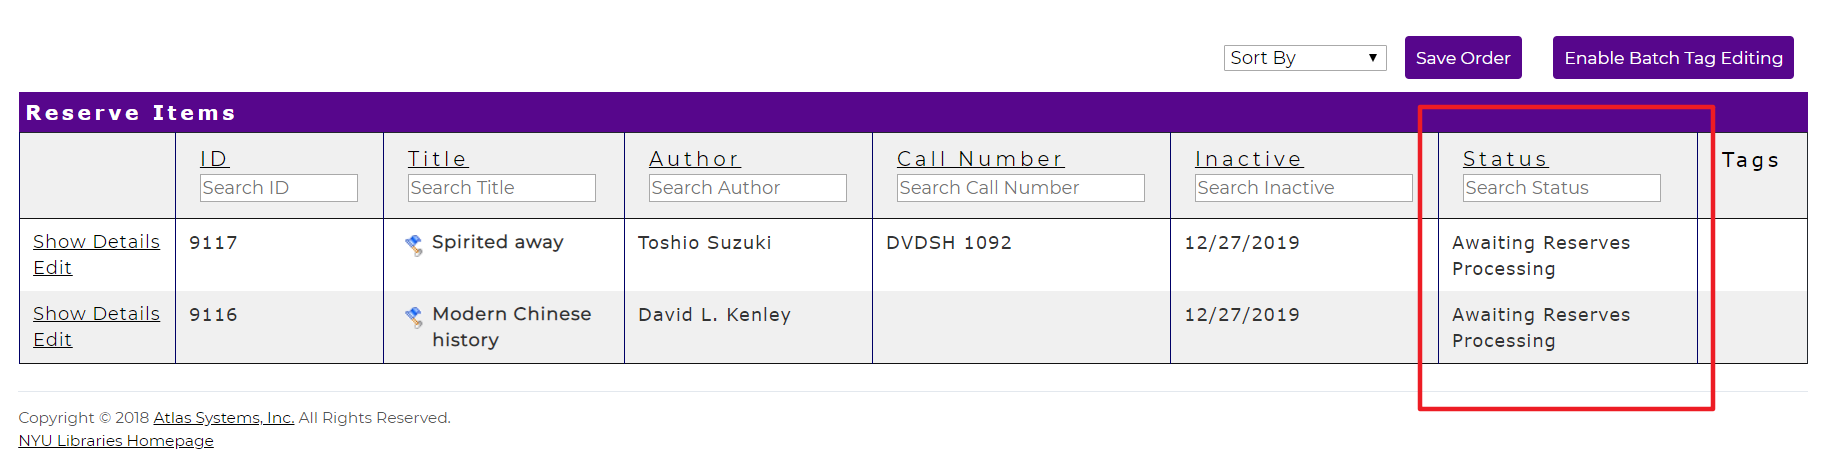
\includegraphics[width=\textwidth]{status}
    \caption{Check Status}
    \label{fig:status}
\end{figure}
\vspace*{1ex}

Here is a list of some typical statuses you might see:
\begin{description}
\item[Awaiting Reserves Processing] Request has been submitted and is pending review by Library staff.

\item[Awaiting Textbook Processing] Request has been submitted and is pending review by Library staff. You answered Yes to ``Is this a required book that students must purchase'' 

\item[Item Available Online] Item has been posted and is accessible. If the link to an item is not working, please contact \href{mailto:shanghai.reserves@nyu.edu}{shanghai.reserves@nyu.edu} as soon as possible.

\item[Item Available at Reserve Collection] Physical item has been processed, and is available at the NYUSH Library Reserve Collection.

\item[Item Activation Pending] Item has been submitted, processed, and will be available on the class start date. If the students need access prior to the course start date, please contact the library.

\item[Awaiting Supply by Instructor] Item has been submitted. This refers to such requests \textbf{1)} that need more information from the instructor, or \textbf{2)} that personal copies need to be received by the Library from the instructor, so that they can be made available on Reserve.

\item[Item Cancelled by Staff] A requested reserve item may be cancelled by Library staff.  Reasons may include not available for purchase.
\end{description}


